\documentclass[../thesis.tex]{subfiles}
\graphicspath{{\subfix{figs/methods/}}}
\addbibresource{biblio.bib}
\pgfplotstableset{
  search path={\subfix{data}},
}
\begin{document}

\chapter{Methodology}
\label{ch:methods}

As shown in the previous chapter, language and society are interwoven in so many ways
that sociolinguistics should be studied most carefully. As scientists, we would like to
establish general principles that explain reasonably well the interactions between society and
language. But to proclaim a law is not enough to establish it: to do so one needs
evidence that supports its claims. That is why we will start this chapter with a
presentation of the empirical aspect of our methods, before introducing the kind of
theoretical modelling that is relevant to this study.

% different media to convey language
% HERE written language exclusively, WHY: our methods, because that's what computers process better
% SO we lose a lot of things that cannot be transcribed, or that are simply not because it would require considerable effort to do so  (accent, intonation), and access to spoken language is much more limited. also lose all non-verbal communication between human


\section{Data}
% TODO: \cite{LazerMeaningfulMeasures2021}? \cite{LazerComputationalSocial2009}?
\subsection{What for?}
To understand a phenomenon, one should first observe it carefully. From the observation,
we may then be able to make representative measurements of reality and encounter
patterns, expected according to our previous knowledge and intuition, or not --- the
latter being the most interesting case. Indeed, since all models are approximations of
reality, it is of utmost importance to be able to find out where they fall short.
Observed data also serve as an essential guide to make sensible hypotheses on which to
build models.

As we are dealing with language, there is no doubt that the centre of our attention
should be the language produced by individuals. It is so omnipresent in our lives that
we can find it anywhere there are human beings, in all kinds of context and in very
different forms. The amount of information that is available is thus colossal. In
comparison, our ability to retrieve it is quite limited.


\subsection{Traditional sources in linguistics}
This was especially true historically. The field of linguistics is centuries-old, and
has relied mostly on written texts and transcriptions of interviews throughout its
history. But despite the considerable efforts that have been made to conserve written records, only a tiny proportion of texts survived through
centuries. The diachronic study of how language evolves with time has thus limited
empirical resources. These sources also used to be only accessible physically, meaning
the researcher would need to travel to collect the data --- or the other way around.
This has a cost and is a source of bias: collecting a geographically uniform
sample is very challenging in these conditions. Less accessible areas and countries
where there was no institution systematically keeping written records are thus vastly
underrepresented.

The texts that were originally in written form present other significant biases. The
texts available to us from the distant past are not representative of the societies of
the time, since only the elites were able to write, and women were essentially barred
from publishing until a couple of centuries ago \cite{SmitterbergEnglishGenres2015}.
Also, for the very nature of the texts that were conserved --- books, legal texts mostly \cite{RissanenHelsinkiCorpus1993,HuSheffieldCorpus2005,DaviesExpandingHorizons2012}
--- colloquial language is almost completely absent from them.

Transcriptions of oral productions may help in this regard. Indeed, they potentially
give access to a different kind of language produced by more diverse speakers. They are
thus very valuable, but unfortunately also very costly to produce, as they require
direct involvement of the researcher in the collection process. This takes considerable
time and effort. This direct involvement also calls for careful procedures to collect
representative samples of languages, and avoid tainting them with the researchers' own
biases \cite{PickfordAmericanLinguistic1956,AlshenqeetiInterviewingData2014}. 

Using the same kinds of sources to study the languages spoken today has become slightly
easier. Travelling to most parts of the world is fast and affordable, and anyway,
collected texts can be digitised and then analysed and shared on large scales. There are
now very large corpora of modern languages, produced in both written
\cite{GrieveCorpusbasedRegional2009,GrieveRegionalVariation2016,BiberCorpusBasedInvestigations1996,McEnerySwearingModern2004}
and spoken
\cite{McEnerySwearingModern2004,SchweinbergerSwearingIrish2018,StenstromTrendsTeenage2002,LabovSocialStratification1966}
forms, that have been shared among researchers for a vast array of analyses. But the
written texts still suffer from a lack of representativity, since, still today, few
social classes publish books, articles or letters. As for interviews, although they are
still highly relevant for the access they provide to spoken language, conducting and
transcribing them faithfully still remains time-consuming. Hence the reduced size of the
oral speech corpora, which are also almost exclusively in English.


\subsection{New sources from online media}
The telecommunication age has brought great promise for the collection of natural
language data. As we already mentioned, sharing information and texts has been made much
easier. But more importantly, the very nature of the new channels of
communication that have been opened allow for systematic collection of natural speech,
both in spoken and written forms. Technically, a mobile network operator can record
calls, and an internet provider or a social media platform can record text sent through them
--- when not end-to-end encrypted. As these media become more and more globally
accessible to people, gone should be the issues of sample representativity, and much
easier should be the collection of linguistic data overall.
% It would then seem we have built a perfect world for linguistics research with these masses of data being collected through every online interaction.

There are two major caveats to mention here though. First, the systematic collection of
such data opens up the potential for serious privacy violations. That is why the
majority of countries have extensive legislation to regulate the collection, processing
and sharing of telecommunication data. Whether all communication service providers
actually abide by these laws internally is doubtful
\cite{GDPREnforcement,GDPRFines2023}, but regardless, they cannot carelessly share
private data with researchers. This brings us to the second caveat: these data are owned
by private companies. There is little to no incentive for them to share their data, and
especially if it requires efforts from them to anonymise the data or make sure that the
use that is made of them does not breach privacy laws. That is why, when they do open
channels for sharing them, they are almost always paid. Further, even with good will,
respecting the privacy of individuals when processing their data is far from trivial. It
has been shown repeatedly that anonymisation is tricky, as researchers managed
to de-anonymise some public datasets
\cite{NarayananRobustDeanonymization2008,GambsDeanonymizationAttack2014}. In order to
conduct research that is both ethical and legal, researchers dealing with such data thus
have to take very particular care \cite{OhmBrokenPromises2009a,KulkBraveNew2012}.

All in all, the advent of telecommunication has not proven to be the panacea for
linguistic data that some may have hoped for. But there is still more linguistic
material to study than ever, as demonstrated by the multiplication of the number of
works in the field of computational (socio)-linguistics
\cite{NguyenComputationalSociolinguistics2016}. These have drawn form a variety of
sources, like blogs \cite{NguyenAuthorAge2011,SchlerEffectsAge2006}, online forums
\cite{BaruaWhatAre2014,GarleyBeefmovesDissemination2012,NguyenAuthorAge2011}, online
reviews
\cite{HovyUserReview2015,Danescu-Niculescu-MizilNoCountry2013,OtterbacherInferringGender2010},
or a certain microblogging website called Twitter \cite{MocanuTwitterBabel2013,AlshaabiStorywranglerMassive2021,CodyClimateChange2015,ZamalHomophilyLatent2012,LiaoLifetimeLexical2014}.


\subsection{The case of Twitter}

The biggest source of data we have used throughout this thesis is Twitter. Twitter is a
microblogging website where people can register to share and view short posts called
Tweets. In them, they can write, mention another user, share images, videos or links to
other websites. The platform is called a \emph{micro}blogging website because these
posts cannot exceed 280 characters (140 before 2017). Tweets
can have a public geotag if the user wishes to include one, which is suggested to the
user when they tweet with their device's GPS turned on. Tweets can be of four kinds:
\begin{itemize}
  \item a simple post that appears on the user profile and is shown on the homepage of
  all the users following this user, which is what people generally refer to with the
  term \emph{Tweet};
  \item a reply to another post, which can be seen by anyone but only shown on the
  homepage of the users involved in the conversation;
  \item a repost to one's profile, to share a Tweet that is already posted (which can be
  one's own), called \ac{RT};
  \item a retweet but with some added text commenting on the quoted post, called
  \ac{QRT}.
\end{itemize}
There are many ways to interact with others, and Twitter thus hosts a huge network of
inter-user interactions. It is one of the most popular online social media, with
hundreds of millions of users worldwide. In the US, for instance, since 2015, more than
\SI{20}{\percent} of the population uses the platform \cite{AuxierSocialMedia2021}. Other
than in the US, it is also popular in many countries globally, although with a slight
bias towards developed, western countries \cite{HawelkaGeolocatedTwitter2014}. Even
though only around \SI{1}{\percent} of Tweets are geotagged
\cite{MorstatterSampleGood2021}, when only counting users who tweet with a geotag, in
around 80 countries there is more than one Twitter user for ten thousand inhabitants
\cite{MocanuTwitterBabel2013}. Hence why Twitter has been extensively used for the
analysis of geographically-embedded text
\cite{ArthurHumanGeography2019,BokanyiRaceReligion2016,BokanyiScalingWords2019,GoncalvesCrowdsourcingDialect2014,GoncalvesLearningSpanish2016,GoncalvesMappingAmericanization2018,
GrieveMappingLexical2019,HuangUnderstandingRegional2016,KoyluUncoveringGeoSocial2018,MocanuTwitterBabel2013,NguyenAudienceUse2015,LamannaImmigrantCommunity2018},
and why we do so in this thesis as well. In the following, we will thoroughly present the
steps we take to leverage Twitter as a source of geotagged text.


\subsubsection{Accessing the data}
A major advantage of Twitter for academic research is how open the platform is to giving
access to its data to researchers. One can send automatic queries to Twitter for data
through their public \ac{API} \cite{TwitterAPI}. In these queries, one can specify rules
to, for instance, retrieve all the Tweets posted in a given country, in a given time
period, or which contain some given text. All the Twitter data we have used throughout
this thesis was retrieved from the filtered stream endpoint of the Twitter \ac{API}
\cite{TwitterAPIa}. They are all geotagged Tweets posted between 2015 and 2021, both
years included, without any geographic restriction, which implies that, a priori, they
could have originated from anywhere in the world.

We show in \cref{fig:tweet_data} an example of the data we can have for each Tweet.
There are two fields in these data that particularly interest us for the works we will
present in the next part and that need careful processing: the textual content of the
Tweet (in \texttt{"text"}) and its geotag (in \texttt{"geo"}). Next, we detail the usual
steps we take to process these. 
\captionsetup[subfigure]{position=top,textfont=normalfont,singlelinecheck=off,justification=raggedright}
\begin{figure}
  \centering
  \subfloat[][]{
    \label{subfig:tweet}
    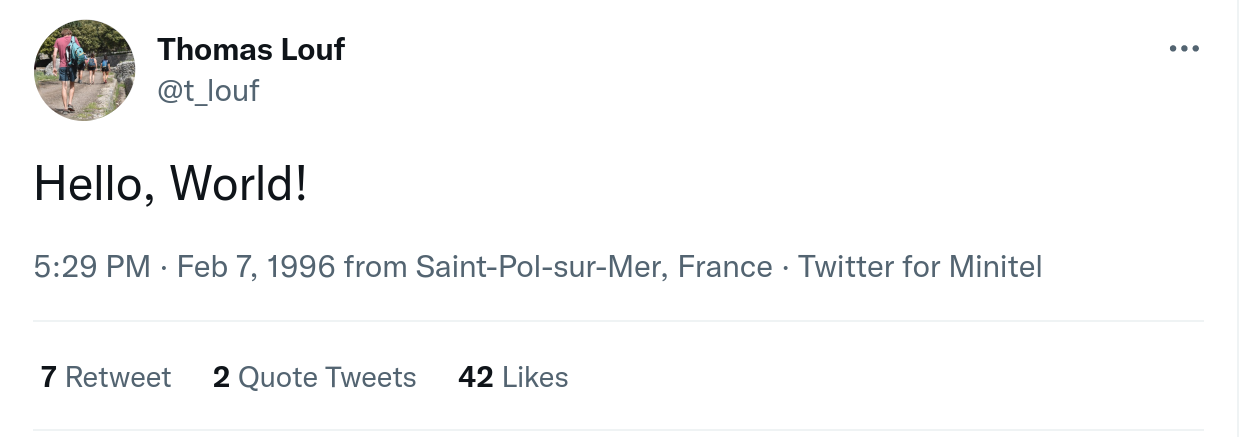
\includegraphics[width=0.95\textwidth]{tweet.png}}
  \\
  \subfloat[][]{
    \label{subfig:annotated_tweet}
  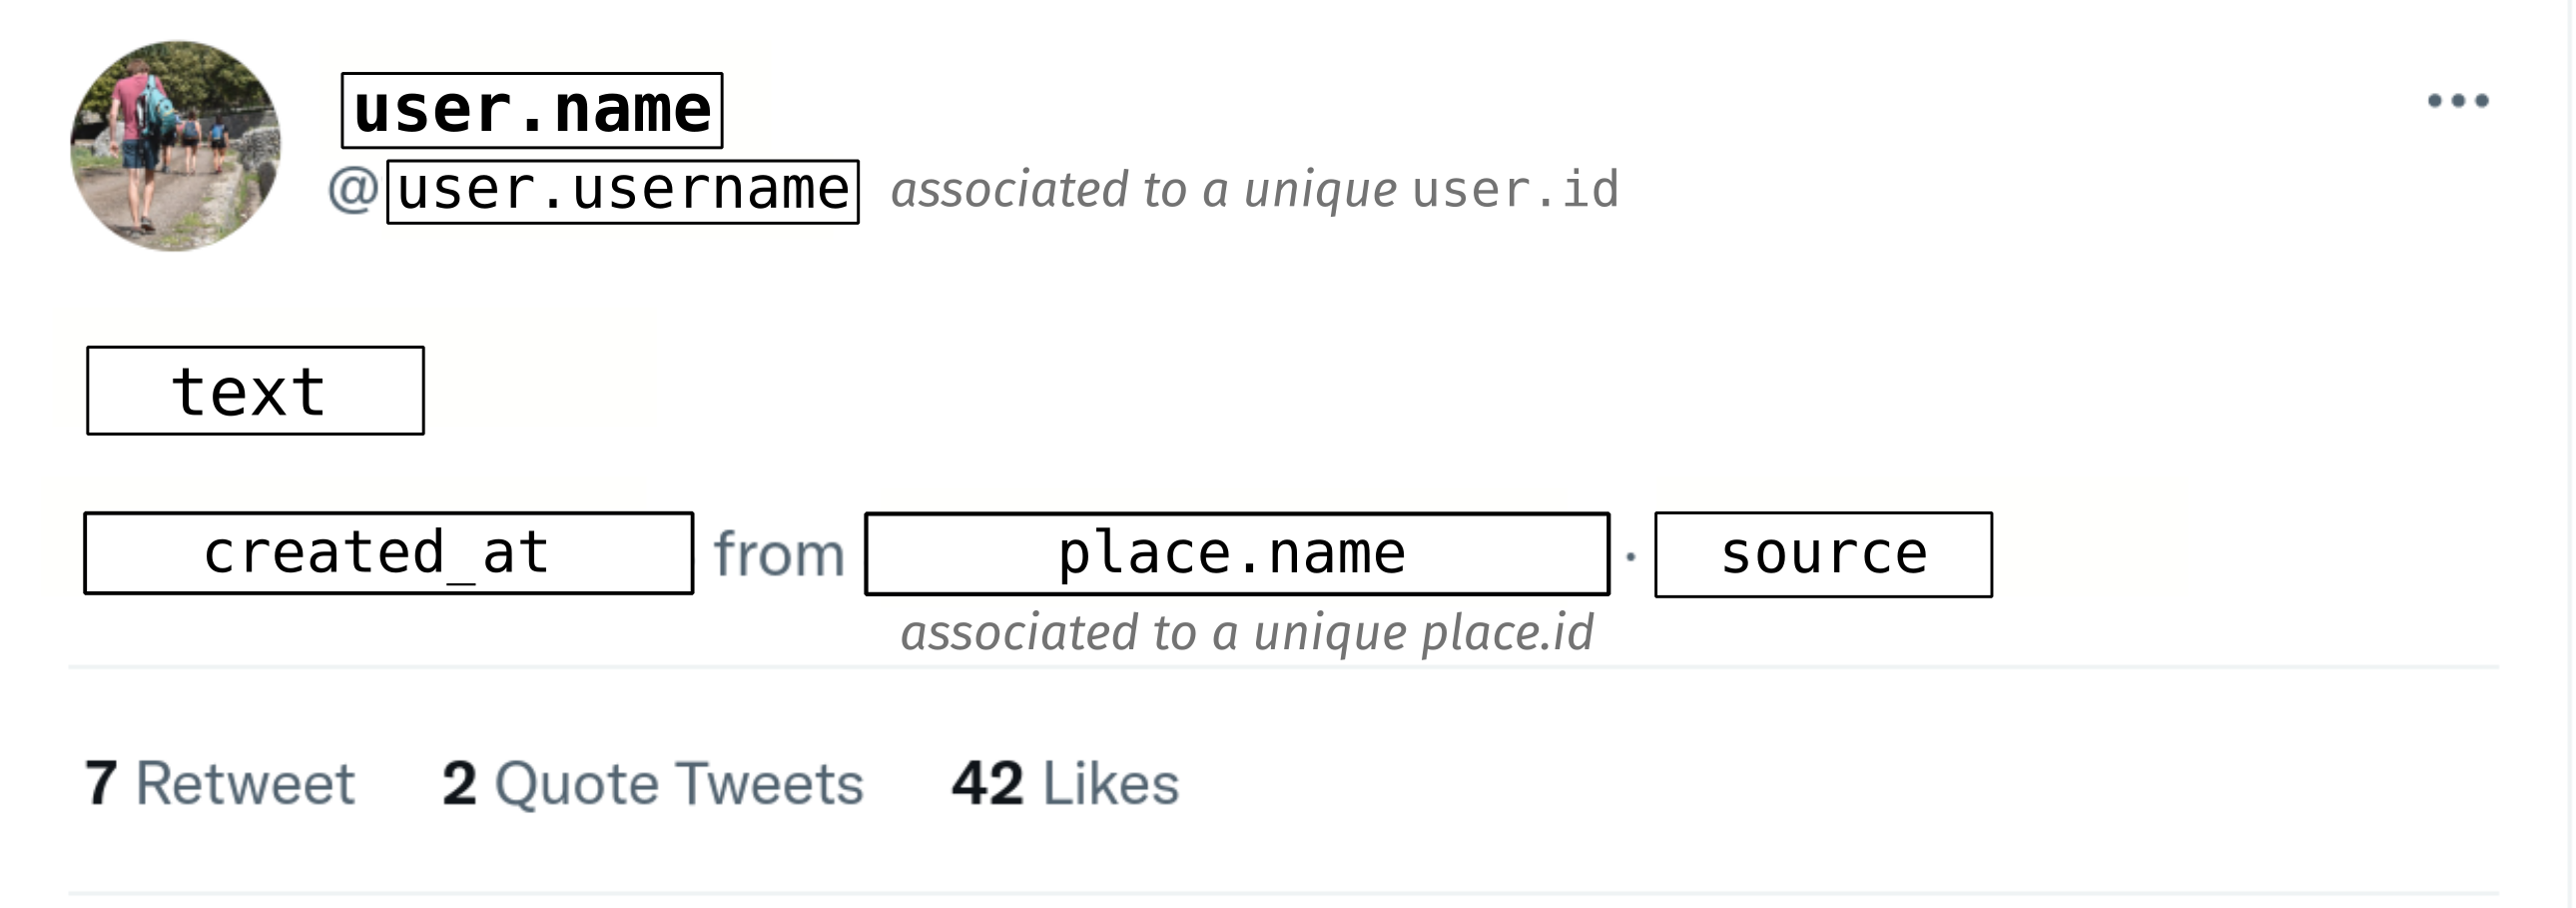
\includegraphics[width=0.95\textwidth]{annotated_tweet.png}}
  \\
  \begin{SubFloat}{\label{subfig:json}}
    \begin{minipage}[b]{0.95\linewidth}
        \begin{lstlisting}[frame=single,xleftmargin=5mm]
{
  "id": "1234567890",
  "text": "Hello, World!",
  "created_at": "1996-02-07T04:29:05.000Z",
  "geo": {
    "place_id": "f68f3d5396bd681c",
    "coordinates": {
      "type": "Point",
      "coordinates": "[2.3295, 51.0249]"
    }
  },
  "source": "Twitter for Minitel",
  "user": {
    "id": "123",
    "username": "t_louf",
    "name": "Thomas Louf"
  }
}
      \end{lstlisting}
    \end{minipage}
  \end{SubFloat}
  \caption[]{A Tweet data. We show \subref{subfig:tweet} an example Tweet as displayed
  on Twitter and \subref{subfig:annotated_tweet} a version annotated with the name of the
  fields in \subref{subfig:json} the data as it would be sent by the \ac{API}, which is
  simply text formatted in a dictionary-like structure (JSON).}
  \label{fig:tweet_data}
\end{figure}


\subsubsection{Text processing}
\label{sec:method_text_process}
Since we are interested in the speech produced by users, we need to clean parts of the
text which cannot be considered as natural language production. Those are the URLs,
mentions of other users (in the form \texttt{@username}) and hashtags (in the form
\texttt{\#topic}). It is not completely obvious that the latter should be discarded
though. Hashtags are used on Twitter to aggregate Tweets by topics. It is an important
feature of the website, whose aim is to enable users to easily find the Tweets of other
users discussing similar topics, or inversely to make one's Tweets more discoverable by
others, and to see real time trends on the platform. Hence, there can be completely
different motivations behind writing a hashtag: to actually tag a Tweet with one or more
topic, to promote the Tweet, or simply follow a trend. Thus, the content of hashtags can
deviate significantly from normal speech \cite{PageLinguisticsSelfbranding2012}. It is
therefore safer to discard hashtags entirely, which is no issue as long as we can
collect enough textual content without them anyway. We actually made some measurements
in our Tweets' database to see if that was the case. We took several random samples of a
million Tweets each, stripped them of URLs and mentions, and then computed the ratio of
characters within a hashtag compared to the total number of characters left in those
Tweets. This proportion was found to be consistently below \SI{5}{\percent}. We thus
consider the precaution of stripping hashtags off of Tweets worth taking. One last kind
of element that we discard are source-dependent. We will not go into details --- our
text-processing code is freely available online anyway \cite{LoufWordsuse2023} --- but,
for instance, when a Tweet was sent from Foursquare, we strip all location-related
content, which can be located after either a \texttt{``I'm at''} or \texttt{``( @ ''}
string.

In practice, all the elements cited above are stripped off of Tweets using regular
expressions. After this cleaning step, for what follows we then keep only the Tweets
still containing at least four words. The next important step that was crucial to all
our works was to infer the language the Tweets are written in. To do so, we leverage a
trained neural network model for language identification: the Compact Language Detector
\cite{SalcianuCompactLanguage2023}. It was designed as part of Chromium-based web
browsers to detect the language web pages are written in in order to make translation
suggestions to users, and it is now openly accessible. Its output is a language
prediction along with the confidence of the model. Whenever we focus on a language, we
thus keep Tweets which are tagged in that language with a confidence above
\SI{90}{\percent}.

We have now described the basic steps of text pre-processing that are recurrent in our
works: out of it we get the Tweets for which we could reliably assign a language,
for which we kept only the text that can be considered the author's natural language production.


\subsubsection{Inferring geolocation}
\label{sec:method_geoloc}
The steps presented above allow us to measure linguistic features of interest from our
Tweets. A next step we usually take is to map those geographically. We are
able to do so thanks to the information contained in the \texttt{"geo"} field of a
Tweet, an example of which is shown in \cref{fig:tweet_data}. This example is actually a
particular case, because of the presence of the \texttt{"coordinates"} field. This gives
precise GPS coordinates of the location of the device used to send out the Tweet: a
longitude, latitude pair. It is present in a Tweet's metadata when the device's GPS is
enabled \emph{and} when the user opted in for precise location tagging in the parameters
of the application. As this setting is opt-in (so off by default), very few users
actually have this enabled: from our measurements, roughly between $10$ and
\SI{20}{\percent} of those who posted with their GPS enabled between 2015 and 2019,
depending on the country. This setting has been in place since 2015, which is the
starting year of the datasets we have used throughout this thesis. So when a user
has enabled their device's GPS but has disabled precise geotagging, this
\texttt{"coordinates"} field is absent, how do we then infer geolocation? In this majority
case, the geotag we have is the \texttt{"place\_id"} we show in the example. This
identifies a place: a specific, named location, which can be of different scales:
\begin{itemize}
    \item a country,
    \item an administrative unit: province, region or department for instance,
    \item a city,
    \item a \ac{POI}: any kind of public place: restaurant, school, event venue, etc.
    These are represented by a point, so Tweets tagged with a \ac{POI} can be considered
    similarly to the ones with coordinates.
\end{itemize}
When a user tweets with their device's GPS activated, a place (usually the city they
tweet from) is selected by default, and they can switch to another one from a list of
close-by places. These places were fed to Twitter by Foursquare
\cite{FoursquarePlaces2019} (among others), which provides data down to a \ac{POI} level
for more than 190 countries. The geographical extent of places other than \acp{POI} is
defined by bounding boxes.

To map linguistic features, Tweets must be attributed to the geographical areas of
interest of the study. These may be defined by administrative boundaries (US counties,
for example) or by us (a regular grid of cells of equal area, for instance). As ``area''
is an ambiguous term that can also refer to the measure of the size of a surface, in the
following we will refer to these areas only by the term \emph{cells}. So, when a Tweet
has GPS coordinates or a \ac{POI} as a geotag, the attribution is straightforward: there
can be only one matching cell. When it has a place defined by a bounding box, it is not
so trivial. The naive approach would be to take the centroid of the place and attribute
to the cell containing it. This is problematic, though. As the cells to match are not
necessarily regular, this method does not systematically match the place to the cell
with the most overlap. A less naive approach would then consist in computing the area of
overlap for every candidate cell and match to the one with biggest such area. This would
still be an all-or-nothing attribution though. What if the place has \SI{51}{\percent}
of its area in one cell and \SI{49}{\percent} in another? It would not be reasonable to
attribute that Tweet to the first cell only. To account for the uncertainty we have when
doing this cell matching, we thus rather do a partial attribution. We attribute the
Tweet to possibly more than one cell, with ratios defined by the ones of the place's
area that lies within each cell. For the example above, and when computing a basic
metric like a count, this means that we attribute \SI{51}{\percent} of the count to one
cell and \SI{49}{\percent} to the other. Because the sizes of places span orders of
magnitude, some may intersect many cells. There can then be so much uncertainty in the
actual geographic origin of the Tweet that it is preferable to discard it. Our criterion
here is that when the four cells which contain most of the place's area put together do
not contain more than \SI{90}{\percent} of its total area, the place, and all the Tweets
assigned to it, are discarded.

As the activity of Twitter users was found to follow a log-normal distribution spanning
almost four orders of magnitude, as shown in \cref{fig:distrib_user_acty}, it can be
preferable to compute metrics at the user level.
Indeed, at the Tweet level, the linguistic behaviour
of the most active users could overshadow the one of the many, less active users.
\begin{figure}[hb]
\centering
  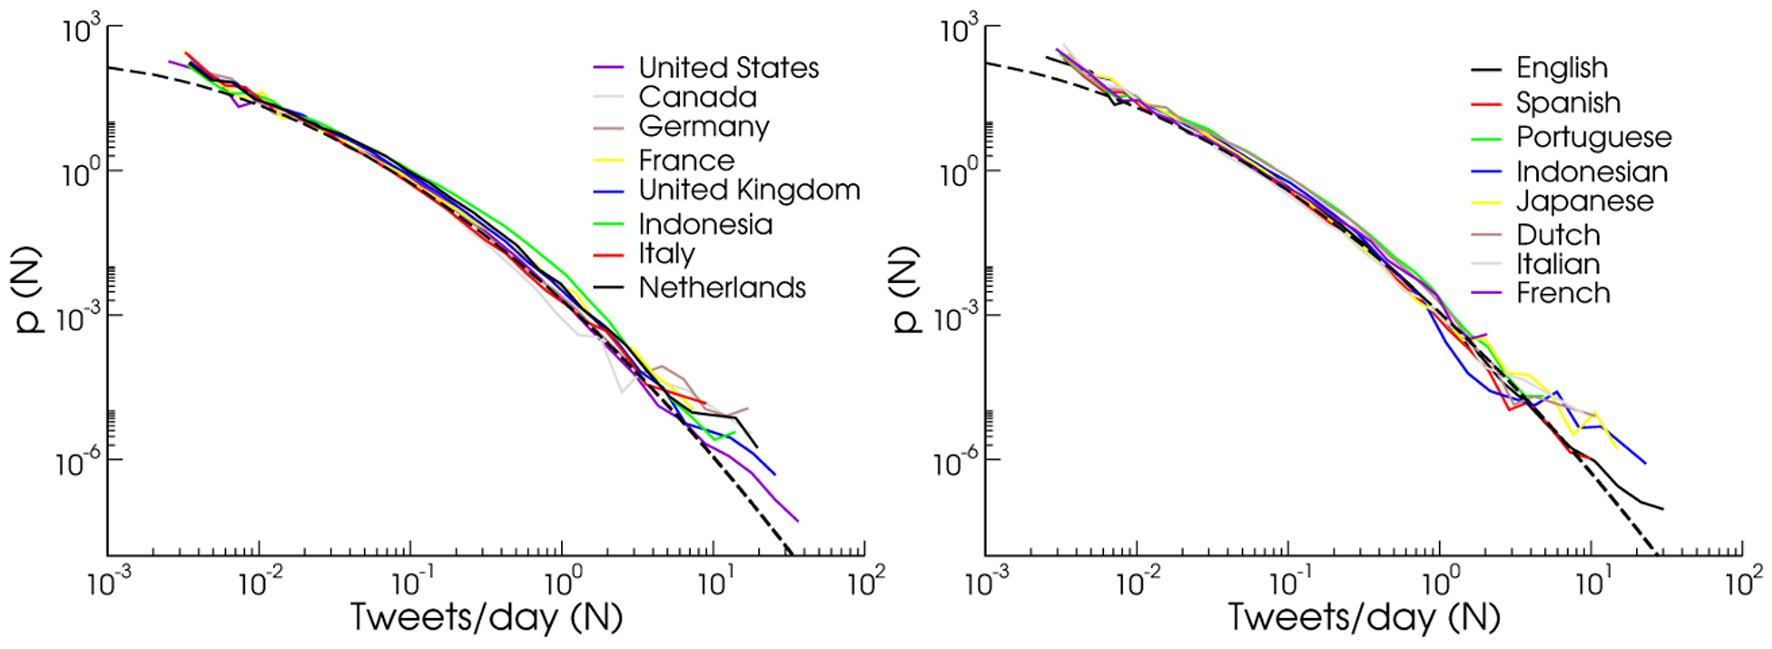
\includegraphics[width=\textwidth]{distrib_user_acty}
  \caption{Distribution of the activity of Twitter users. The probability density $p(N)$
  of user activity (number of daily tweets $N$) grouped by country (left) and language
  (right) is plotted. Different curves collapse naturally, which indicates the presence
  of a seemingly universal distribution of user activity, independent of cultural
  backgrounds. Dashed lines represent log-normal distributions $p(N) \sim 1 / (N \sigma
  \sqrt{2 \pi}) \cdot \exp[-( \ln N - \mu)^2 / 2 \sigma^2]$ with $\mu = -5.16$ and
  $\sigma = 1.67$ on the left and $\mu = -5.55$ and $\sigma = 1.70$ on the right.
  Adapted from \cite{MocanuTwitterBabel2013}.}
  \label{fig:distrib_user_acty}
\end{figure}

Individuals are mobile but for the vast majority they have a preferred location, namely
their place of residence. That is why we often strive to attribute a cell of residence
to the users in our datasets. To explain the heuristics we defined for residence
attribution, let us first formalise some notation. For each user $u$, there are two
counts we get directly from their Tweets: the number of them with GPS coordinates that
fall in cell $c$: $n_{u, c}^{\text{GPS}}$, and those without coordinates but tagged as
being from place $p$: $n_{u, p}$.  We wish to compute $r_{u, c} \in \mathbb{R}^+$, the
weighted count of Tweets of user $u$ in cell $c$. It can be decomposed into the contributions of
those with GPS coordinates, $n_{u, c}^{\text{GPS}}$, and of those tagged with a place, $r_{u,
c}^{\text{P}}$:
\begin{equation}
  r_{u, c}
    = n_{u, c}^{\text{GPS}} + r_{u, c}^{\text{P}}.
\end{equation}
Denoting $A_p$ and $A_{p \cap c}$ the areas of the place $p$ and of the intersection
between $p$ and $c$, respectively, the partial attribution described above yields:
\begin{equation}
  r_{u, c} = n_{u, c}^{\text{GPS}} + \sum_p n_{u, p} \frac{A_{p \cap c}}{A_p}.
\end{equation}
We provide an illustration for this cell attribution in
\cref{fig:tweet_partial_attrib_diagram}.
\begin{figure}[hb]
\centering
  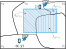
\includegraphics{tweet_partial_attrib_diagram}
  \caption{Diagram illustrating how geotagged Tweets are attributed to cells. A first
  Tweet has GPS coordinates $(x, y)$ attached to it, and can thus be directly attributed
  to $c_4$. It thus increments $n_{u, c_4}^{\text{GPS}}$ by 1. Another is tagged in
  place $p$, defined by a bounding box, shown in blue. It will be attributed partially
  to $c_2$, $c_3$ and $c_5$, with weights equal to the ratio of overlapping area
  $A_{p \cap c_k} / A_p$, thus incrementing $r_{u, c_k}^{\text{P}}$ by these
  values for the three cells.}
  \label{fig:tweet_partial_attrib_diagram}
\end{figure}

To attribute a cell of residence to each user $u$, we first only consider cells where
$r_{u, c} \geq 3$ and $r_{u, c} / \sum_{c'} r_{u, c'} \geq 0.1$. We also compute
$r_{u,c}$ considering only Tweets posted at nighttime (from 6pm to 8am), that we denote
$r_{u, c}^\text{NT}$. Among those left, the cell of residence $c^*$ is then the one such
that $r_{u, c^*}^\text{NT} / \sum_{c'} r_{u, c'}^\text{NT} \geq 0.5$, if any. This
roughly means that we impose that a user must have tweeted at least three times and at
least \SI{10}{\percent} of the time from that cell, and that at night the majority of
their Tweets were from there. All users for whom a cell of residence cannot be
attributed are subsequently discarded from the analysis. The three thresholds given
above were chosen because we believe them to be reasonable, but they may be adjusted to
each analysis, and also tweaked for sensitivity analyses. They are summarised along with
other criteria in \cref{tab:twitter_criteria}.


\subsubsection{Selecting relevant users}
\label{sec:method_users_select}
As we are interested in the natural speech produced by individuals, we actually start
our analyses by filtering out users whose behaviour resembles that of a bot. We first
eliminate those tweeting at an inhuman rate, set at an average of ten tweets per hour
over their whole tweeting period. Then, we only keep those who tweeted either from a
Twitter official app, Instagram, Foursquare or Tweetbot (a popular third-party app).
These were selected because they are significantly popular among real users. Also,
consecutive geolocations implying speeds higher than a plane's (\SI{1000}{\kilo \meter
\per \hour}) are detected to discard users. The final filter is optional: when we wish
to only keep residents of the region considered, we impose for a user to have tweeted
from there in at least three consecutive months. Again, the values for the criteria
given above were set as they were deemed reasonable and allowed us to safely discard
problematic users. A summary of these values is given in \cref{tab:twitter_criteria},
while \cref{tab:region_counts} gives the counts of Twitter users in our dataset that we
found to be locals of one of several multilingual regions, using these criteria.

\begin{table}[h]
  \centering
  \begin{tabular}{
    @{}
    p{0.2\textwidth-2\tabcolsep}
    >{\raggedright}p{0.45\textwidth-2\tabcolsep}
    >{\centering\arraybackslash}p{0.35\textwidth-2\tabcolsep}
    @{}
  }
    \toprule
    Language detector & Minimum length of Tweets after cleaning & 4 words \\
    & Minimum confidence of the model & \SI{90}{\percent} \\
    % \midrule
    \addlinespace
    Relevant places & Maximum number of overlapped cells & 4 cells contain \SI{90}{\percent} of its area \\
    % \midrule
    \addlinespace
    \multirow[t]{3}{0.2\textwidth-2\tabcolsep}{Residence cell} & Minimum activity in cell & 3 Tweets \\
    & Minimum proportion of activity in cell & \SI{10}{\percent} \\
    & Minimum proportion of nighttime activity in cell & \SI{50}{\percent} \\
    % \midrule
    \addlinespace
    Real users & Maximum tweeting rate & 10 Tweets per hour \\
    & Maximum speed & \SI{1000}{\kilo \meter \per \hour} \\
    & Minimum period of activity & Once a month for 3 consecutive months \\
    \bottomrule
  \end{tabular}
  \caption{Criteria used for Twitter data preprocessing. They are applied over the whole
    tweeting span of a user in our dataset, which, in this work, is at most from the
    years 2015 to 2021, both included. This means for example that the tweeting rate is
    the total number of Tweets posted by a user divided by the amount of time that
    passed between their first and last Tweet in the dataset.}
  \label{tab:twitter_criteria}
\end{table}

\begin{table}[h]
  \centering
  \pgfplotstabletypeset[
    column type=l,
    % assign column name/.style={/pgfplots/table/column name={\textbf{#1}}},
    every head row/.style={after row=\midrule, before row=\toprule},
    every last row/.style={after row=\bottomrule},
    columns/regionname/.style={
      string type,
      column name=Region
    },
    columns/countlocals/.style={
      string type,
      column name={\text{Number of local Twitter users}},
      column type={S}
    },
  ]
  {count_locals.csv}
  \caption{ Number of Twitter users found to be residents and speaking a local language
    between 2015 and 2019 in several multilingual regions.}
  \label{tab:region_counts}
\end{table}

\subsubsection{Caveats}
No data source is without bias, and Twitter is no exception. First, at the global scale,
as we already mentioned, Twitter is more representative of people living in western,
developed countries with widespread access to the Internet
\cite{HawelkaGeolocatedTwitter2014,MocanuTwitterBabel2013}. In terms of more local
geographical biases, densely populated urban areas are usually overrepresented
\cite{MisloveUnderstandingDemographics2011,JiangUnderstandingDemographic2019,AuxierSocialMedia2021}.
As for demographics, Twitter users are on average younger
\cite{NguyenHowOld2013,AuxierSocialMedia2021,SloanWhoTweets2017}, with more degrees and
income, and more likely to be male
\cite{MisloveUnderstandingDemographics2011,AuxierSocialMedia2021,SloanWhoTweets2017}
than the general population. These biases have to be taken into consideration, and
alleviated whenever possible. For instance, some metrics can be rescaled non-uniformly
across space, matching marginals obtained from the census using \ac{IPF}
\cite{DemingLeastSquares1940,FienbergIterativeProcedure1970}. For instance, as we will
see in \cref{ch:multiling}, we used it when rescaling cell counts of speakers of
different languages in a given region found on Twitter. \Ac{IPF} allowed us to make
their sum over cells by language match a given country's official statistics on overall
number of speakers by language, and also to match the real number of residents of every
cell.



\section{Computational models of natural language}
The increased availability of natural language data has also been followed by the
development of new tools for \ac{NLP}. Rather than an in-depth review, we will here
simply give a very brief overview of the field and mention a few algorithms and tools
that were useful to us throughout this thesis. Nowadays \ac{NLP} has become familiar to
the general public through large language models: deep neural networks with billions of
parameters trained on billions or soon-to-be trillions of tokens. Popular examples are
Open AI's GPT models \cite{BrownLanguageModels2020} Google's BERT
\cite{DevlinBERTPretraining2019} and its derivatives \cite{SanhDistilBERTDistilled2020},
or the BigScience workshop's BLOOM \cite{WorkshopBLOOM176BParameter2022}, with an
increasing number of pre-trained models made freely accessible
\cite{WolfTransformersStateoftheArt2020,MontaniExplosionSpaCy2023}. These kinds of
models are best known for their derivatives optimised for usage as chatbots, but they
have many variants and parts that can serve different functions: lemmatising, that is
finding the base forms of words (like removing plurals or conjugation), classifying
documents, or finding similarity between words and documents by embedding them in a
vector space (with for instance \texttt{word2vec} \cite{MikolovEfficientEstimation2013}
and \texttt{tok2vec} \cite{AngelovTop2VecDistributed2020}, respectively). As said above
in \cref{sec:method_text_process}, and as we will see in the next chapters, these kinds
of models can also be used to detect the language a text is written in. Although they
are very powerful tools to carry out some tasks, their training is very costly
\cite{AnanthaswamyAIBigger2023}, and most of the pre-trained models were trained on
rather formal speech, like blog or news articles. They are thus not always well suited
to analyse social media speech, as the one found on Twitter for instance. Some works
have strived to normalise informal texts to be able to use such tools, but doing so
throws away valuable information \cite{EisensteinWhatBad2013}. Also, \ac{NLP} has
existed for some decades now, and some simpler tools developed further in the past may
sometimes suffice to carry out some tasks. Latent semantic analysis
\cite{DumaisLatentSemantic2004} can be good enough to compute document similarities and
then cluster documents together. It simply consists in computing a matrix of word
frequencies by document, reducing its dimensionality with a singular value
decomposition, thus performing \ac{PCA} \cite{WoldPrincipalComponent1987} to then
cluster documents together based on their cosine similarity. This method can be adapted,
by using a matrix containing a different metric than simple frequencies, or clustering
based on a different method to compute similarity, as we will show in \cref{ch:acr}.
Latent Dirichlet allocation \cite{BleiLatentDirichlet2003} can perform good topic
modelling in some settings. A recent work has shown that algorithms developed to infer
communities in networks can be adapted to provide robust topic modelling and document
clustering at the same time \cite{GerlachNetworkApproach2018}. Our results presented in
\cref{ch:ses_ling}, based on the detection of the use of standard language, are based on
a grammar and spell checker, LanguageTool, which simply performs part-of-speech tagging
before searching for matches of patterns indicating a broken rule of the standard
language. The tools are thus many, but the context in which they are used greatly
conditions their actual power.



\section{Theoretical models}

\subsection{What for?}
We mentioned some models just above, but there is an important distinction to make here
with the models we will describe further down. The former are machine learning models:
they are algorithms that, after being trained on input data, can predict some output
when presented with new data. Hence their name: they are models learnt from data through
an algorithm. They can even learn so much from the data that they can end up having
learned the training data itself, which makes them unusable to make further predictions.
This is what is called over-fitting. But there are many techniques, like regularisation
or cross-validation, that can be used to avoid this pitfall. They can also be so complex
that they become what is known as a black-box model: a model that cannot be interpreted
in terms of the influence of the input variables, and whose behaviour is thus
unpredictable. Again, this issue can be alleviated with methods such as the computation
of Shapley values \cite{ShapleyNotesNPerson1951,StrumbeljExplainingPrediction2014}. But
crucially, what even the best-trained algorithms cannot provide is explanation. Models,
as those we will mention further down, and as understood by most scientists, try to
uncover the mechanisms underlying some observed phenomena. They do not only aim to
predict, but also to lay a fertile ground for further development, and may help
understand other phenomena than the one they were initially intended to explain
\cite{EpsteinWhyModel2008}. Additionally, they are built on explicit assumptions, which
allow to clearly set out their scope of validity. Incidentally, a machine learning model
needs input data to be trained, but how does one select what variables to look for, what
measurements to make, and how? This is again where a theory can help. That is why many
times, throughout the history of science, it was the theory that preceded the empirical
works \cite{EpsteinWhyModel2008}. Theoretical models thus remain invaluable, and rather than a replacement, machine learning models can serve as useful guides in their development by quickly uncovering patterns found in the data. 


\subsection{What kind?}
One of the first things to consider when trying to model a phenomenon is at what level
we wish to study it. % TODO meh
We will here distinguish between two levels: the microscopic and the macroscopic. To
illustrate this distinction, we will take the example of the modelling of language
competition, which has been approached by many physicists and applied mathematicians
with different frameworks
\cite{CastellanoStatisticalPhysics2009,BoissonneaultSystematicInterdisciplinary2021}.

At the macro level, one considers the system of interest as a whole and tries to come up
with equations that describe the dynamics of some global metrics that summarise the
state of the system. In language competition, the system can be a society with many more
internal than external interactions, like a country, and the global metrics can be the
proportions of people speaking each language. One such model that has been very
influential in language competition modelling is the Abrams-Strogatz model
\cite{AbramsModellingDynamics2003}. It considers a group where individuals speak either
language A or B. It captures the fact that, the more people speak A, and the more
prestigious A is in society, the more B speakers will want to switch to A, and
inversely. Its proposal is considered a seminal work in this field for the simplicity of
its formulation, which inspired many further works. The model is defined by a single
equation:
\begin{equation}
  \label{eq:AS_dt}
  \dv{p_A}{t} = (1 - p_A) s p_A^a - p_A (1 - s) (1 - p_A)^a,
\end{equation}
thus describing the evolution with time of the proportions of A speakers $p_A$, which
depends on an exponent $a > 0$ and a factor $s \in [0, 1]$ called the relative status of
language A. When this status has a value above 0.5, A is relatively more prestigious
than B, and the inverse is true when it is below 0.5. The exponent $a$, later on called
(inverse) volatility, controls the effect of social pressure. For instance, in the first
term of equation \eqref{eq:AS_dt}, it controls how much influence the proportion of A
speakers $p_A$ will have on the B speakers --- present in a proportion equal to $(1 -
p_A)$ --- when considering learning A. The lower $a$, or the higher the volatility, the
more importance this term will have, so the easier the switch. A clear advantage of such
a model is its high tractability. First, it is straightforward to fit to existing data,
which is what \citeauthor{AbramsModellingDynamics2003} did with historical data on the
proportion of speakers of Scottish Gaelic, Welsh and Quechua, thus predicting the death
of these languages \cite{AbramsModellingDynamics2003}. Second, it lends itself to
mathematical analysis, which in this instance allowed \citeauthor{VazquezAgentBased2010}
to determine that the model only allowed stable coexistence of two languages for $a > 1$, as shown in \cref{fig:AS_fc_param_space}.
\begin{figure}[hb]
\centering
  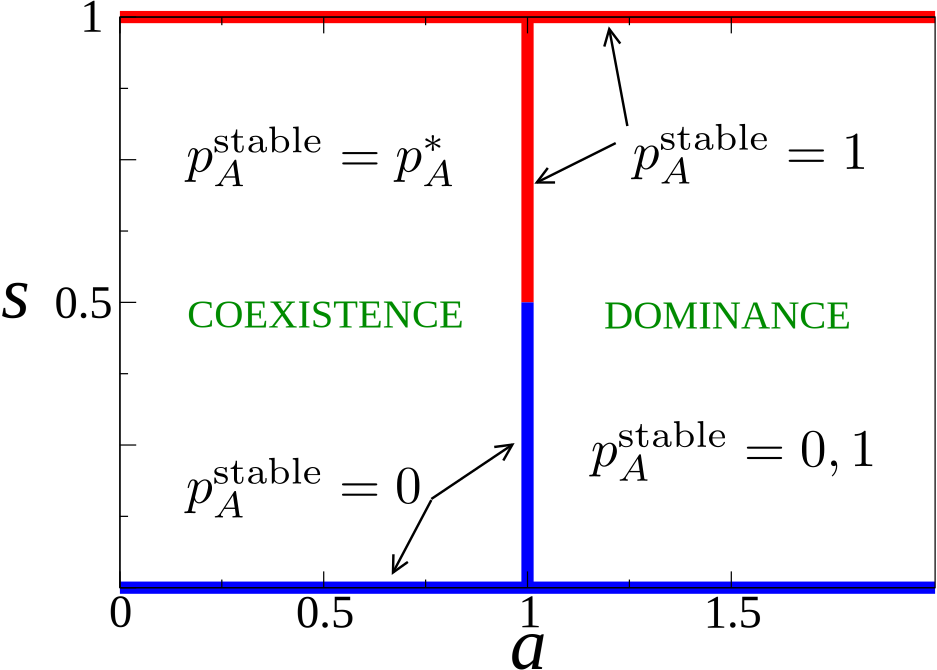
\includegraphics[width=0.6\textwidth]{AS_fc_param_space}
  \caption{Parameter space of the Abrams-Strogatz model. The different stable fixed points are presented, split into two kinds by the $a = 1$ line: coexistence and dominance. In the coexistence region of the parameter space, the stable fixed point is such that $0 < p_A^* < 1$, meaning that the proportions of both A and B speakers are non-null. Adapted from \cite{VazquezAgentBased2010}.}
  \label{fig:AS_fc_param_space}
\end{figure}
Many other models of the same kind have been proposed to understand language shift,
extending previous formulations to consider additional aspects of the problem. Notably,
most subsequent models have incorporated bilingualism, as they included a third
population of bilinguals AB, which may influence the dynamics in different ways. For
instance, including interlinguistic similarity in a model with bilinguals, the latter
may keep a minority language alive when this similarity is high enough
\cite{MiraImportanceInterlinguistic2011}. \Citeauthor{MinettModellingEndangered2008}
have stressed the importance of considering different maximum rates between the
processes of learning and losing a language, as these happen on different timescales,
and argued that individuals cannot transition from being monolingual in a language to
monolingual in another, but rather that they should necessarily go through bilingualism
to make the transition \cite{MinettModellingEndangered2008}.
\Citeauthor{HeinsaluRoleBilinguals2014} tweaked the model, making the bilingual
population also influence the monolinguals to learn the other language
\cite{HeinsaluRoleBilinguals2014}. These three models have greatly inspired our own
modelling endeavour, that we will present in \cref{ch:multiling}. Also of note, several
have taken inspiration from models of interspecies competition from ecology
\cite{PinascoCoexistenceLanguages2006,KandlerEcologicalModels2008,SoleDiversityCompetition2010},
and others have taken the spatial embedding of languages into account as well using
reaction-diffusion-like models
\cite{KandlerDemographyLanguage2009,PatriarcaInfluenceGeography2009,IsernLanguageExtinction2014,ProchazkaQuantifyingDriving2017}.

Instead of a single population, one may consider a metapopulation, that is a population
of populations that may interact with each other as they move around. This has been used
extensively in ecological models to take into account the movements of species for the
dynamics of inter-species competition \cite{HanskiMetapopulationDynamics1998}. It was
used similarly in epidemiology to try to understand how the propensity of individuals to
stay in their home region or to move to others and potentially transmit a disease to
another population may contribute to an epidemic
\cite{SattenspielStructuredEpidemic1995,BalcanModelingSpatial2010,ApolloniMetapopulationEpidemic2014}.
Even closer to our topic, the metapopulation framework has proved useful to study a
model of voting behaviours \cite{Fernandez-GraciaVoterModel2014}. It can thus surely be
adequate to test a sociolinguistic model, and in particular a model of language shift,
as we will show in \cref{ch:multiling}.

While some social aspects can be modelled with some parameters in global equations, or
the mobility of the population can be taken into account in a metapopulation framework,
the social structure itself can hardly be incorporated into these two kinds of model.
That is where the micro approach shines, notably with a class of models called
\acp{ABM}. In such a model, it is not the evolution of the global population that is
modelled, but the evolution of the state of each individual, or agent, in that
population. Their state could be linked to a linguistic variable, or even a set of them.
In the case of language competition, it may be the language(s) they speak. The model
then defines switching rules between states. For instance, one can rewrite the
Abrams-Strogatz model of \eqref{eq:AS_dt} as an \ac{ABM}, writing the following
transition probabilities:
\begin{equation}
  \label{eq:AS_ABM}
  \begin{aligned}
    P(A \rightarrow B) &= (1 - s) (1 - p_A)^a, \\
    P(B \rightarrow A) &= s p_A^a,
  \end{aligned}
\end{equation}
from A to B, and B to A, respectively. Each agent, in function of their current state,
may switch to another, with potentially their own probability. Indeed, if each agent
sees different proportions $p_A$, because they interact with different people, then the
social structure can be reflected in \eqref{eq:AS_ABM}. And from this transition rule,
any kind of social structure can be plugged into the model, from the very basic but
mathematically-tractable complete network, to more realistic social networks from
synthetic models or even real-world data. \Acp{ABM} of language competition have thus
been tested in 2D lattices, small-world networks \cite{WattsCollectiveDynamics1998}, or
synthetic networks with community structure
\cite{CastelloOrderingDynamics2006,MinettModellingEndangered2008,CaridiSchellingvoterModel2013,CastelloAgentbasedModels2013,VazquezAgentBased2010}. They may still allow for analytic study, especially working in the simple case of a complete network of interactions and in mean-field, as these approximations enable to write evolution equations that may provide a good, approximate prediction of the average global trend in the population \cite{VazquezAgentBased2010}. We have here cited works focused on language dynamics, from physicists mainly, but there is a long tradition of leveraging \acp{ABM} in the social sciences, with the seminal works of Axelrod on the dissemination of culture \cite{AxelrodDisseminationCulture1997}, or Schelling's on the emergence of segregation \cite{SchellingDynamicModels1971}.

Despite their nature, one should not expect these models to offer predictions at the
micro, or individual, level. Even though they define rules at this level, they do not
--- or at least should not --- claim that they predict the behaviour of each individual.
Rather, what they try to achieve is chiefly to capture the crucial mechanisms that give
rise to observed global trends \cite{MacyFactorsActors2002}. In that regard they are
thus not so different from models defined at the macroscopic level. What they definitely
bring to the table is how they enable us to study how some properties of the social
structure may matter in sustaining the observed dynamics. We here reference again to the
citation of \citefirstlastauthor{BlommaertSociolinguisticsGlobalization2010} we gave in
the previous chapter, that the world had become more of ``a tremendously complex web of
villages towns, neighbourhoods, settlements'' than a simple global village, where
everyone is perfectly connected. Then to understand the ``complexity'' that emerges from
this, a model that describes dynamics that can happen on any kind of complex network of
interaction is invaluable. For example, \acp{ABM} can provide insights into questions
with a long history in social sciences \cite{LatanePsychologySocial1981}, such as: does
this cultural feature persist in part of the population partly because it creates a
sense a group identity that binds people together? Will the increasing number of
contacts between these populations tend to smooth out differences between them?


\section{Source materials and tools}
Following the principles of open science, throughout my thesis, I have made all source
materials for my results openly accessible, whether they are codes\footnote{Hosted on
GitHub at \url{https://github.com/TLouf}} or datasets\footnote{Hosted on figshare at
\url{https://figshare.com/authors/Thomas_Louf/9441395}}, including this very
manuscript's\footnote{Hosted at \url{https://github.com/TLouf/phd-thesis}}. Equally importantly, I believe, I have strived to use almost exclusively free
and open source software in my work. I cannot realistically cite here all projects I
have relied on to carry out my work, but I can cite a few central ones. I wrote all my
code in the Python 3 programming language, using libraries such as
NumPy~\cite{HarrisArrayProgramming2020},
pandas~\cite{teamPandasdevPandas2020} or
GeoPandas~\cite{JordahlGeopandasGeopandas2020}. In their vast majority, figures
presented here were prepared with Matplotlib~\cite{HunterMatplotlib2D2007}, and
sometimes edited, or entirely drawn, with Inkscape\footnote{Available at
\url{https://inkscape.org}}.

This document was prepared using \LaTeX\ with the \texttt{classicthesis}
style\footnote{Hosted at \url{https://www.ctan.org/pkg/classicthesis}}, and the LaTeX
Workshop extension\footnote{Hosted at \url{https://github.com/James-Yu/LaTeX-Workshop}}
of Visual Studio Code, and the references were managed using Zotero\footnote{Available
at \url{https://www.zotero.org}}.
% managed the references cited in this work with Zotero https://www.zotero.org/



\end{document}
